
\chapter{문서 만들기} 
본 장에서는 실제 문서를 작성하기 위해 필요한 다양한 명령어들을 소개합니다. 이렇게까지 친절할 필요가
있을까하는 의문이 강하게 듭니다.

\section{본문 내용 작성}
\subsection{글꼴 바꾸기}
\subsubsection{진하게}
\begin{verbatim}
    \textbf{진하게 표시할 글자}
\end{verbatim}

\subsubsection{나눔고딕체 사용}
\begin{verbatim}
    \textsf{나눔고딕체로 표시할 내용}
\end{verbatim}

\subsection{그대로 표시}
표기방식에 설명된 파일/경로명, 사용자 입력 및 소스코드 등은 다음과 같이 작성합니다.
\begin{verbatim}
    \begin{verbatim}
        내용 작성
    \end{vertim}
\end{verbatim}

\subsection{주의 또는 참고사항}
\begin{verbatim}
    \begin{notice}
        내용 작성
    \end{notice}
\end{verbatim}

\section{이미지 넣기}
문서에 그림을 넣는 작업의 간단한 예시입니다. 그림과 관련한 자세한 내용은 아래 링크의 그림넣기 장을
참고하시기 바랍니다. \\

http://willkwon.dothome.co.kr/wp-content/uploads/2018/01/lecture3.pdf

\subsection{이미지 넣기 명령}
\begin{verbatim}
    \begin{figure}[h!]  % t! = top, h! = here, b! = bottom
        \centering            % 이미지 정렬
        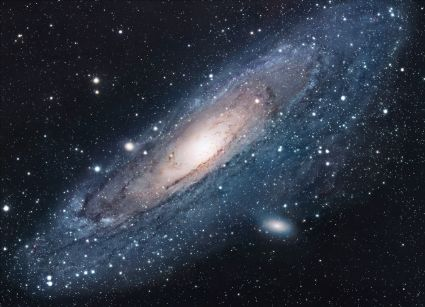
\includegraphics[scale=2]{images/universe}
        \caption{그림 아래에 표시될 캡션}
        \label{fig:universe}   %이미지 참조를 위한 레이블
    \end{figure}
\end{verbatim}

\begin{figure}[h!] 
    \centering            % 이미지 정렬
    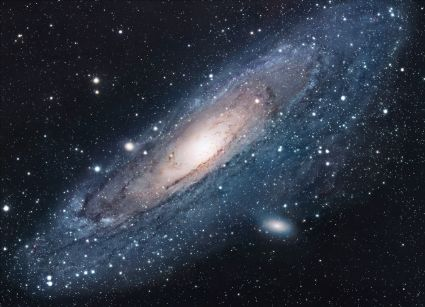
\includegraphics[scale=2]{images/universe}
    \caption{그림 아래에 표시될 캡션}
    \label{fig:universe}   %이미지 참조를 위한 레이블
\end{figure}

\subsection{이미지 레이블 참조}
문서에 넣은 이미지에 대한 레이블은 다음과 같이 참조할 수 있습니다. 이렇게 한 번 작성된 참조는
실제 그림 번호가 바뀌더라도 수정할 필요가 없습니다. 개인적으로 \LaTeX의 최대 장점이라 생각합니다.

\begin{verbatim}
    관련된 내용은 그림 \ref{fig:universe}을 참고하시기 바랍니다. 
\end{verbatim}

관련된 내용은 그림 \ref{fig:universe}을 참고하시기 바랍니다.

\section{표 만들기} 
문서에 표를 작성하는 작업의 간단한 예시입니다. 표 작성과 관련한 자세한 내용은 아래 링크의 표 넣기
장을 참고하시기 바랍니다. \\

http://willkwon.dothome.co.kr/wp-content/uploads/2018/01/lecture3.pdf \\

표를 만드는 작업은 상당히 \LaTeX에서 상당히 까다로운 작업으로 표를 생성해주는 서비스를 이용하는 것도
좋은 방법입니다.

https://www.tablesgenerator.com/

\subsection{표 만들기 명령}
\begin{verbatim}
    \begin{table}
        \begin{tabu}{X | X | X | X} \hline
            \textbf{구분} & \textbf{항목} & \textbf{내용} & \textbf{비고} \\ \hline
                구분1 & 항목1 & 내용1 & 비고1 \\ \hline
                구분2 & 항목2 & 내용2 & 비고2 \\ \hline
            \end{tabu}
            \caption{표에 대한 설명}
            \label{tab:table_01}
    \end{table}
\end{verbatim}

\begin{table}[h!]
    \begin{tabu}{X | X | X | X} \hline
        \textbf{구분} & \textbf{항목} & \textbf{내용} & \textbf{비고} \\ \hline
            구분1 & 항목1 & 내용1 & 비고1 \\ \hline
            구분2 & 항목2 & 내용2 & 비고2 \\ \hline
        \end{tabu}
        \caption{표에 대한 설명}
        \label{tab:table_01}
\end{table}

\subsection{표 레이블 참조}
작성된 표에 대한 레이블도 그림과 동일한 방법으로 참조할 수 있습니다.

\begin{verbatim}
    관련된 내용은 표 \ref{tab:table_01}을 참고하시기 바랍니다. 
\end{verbatim}
관련된 내용은 표 \ref{tab:table_01}을 참고하시기 바랍니다. 

\section{각주 넣기}
문서 내의 특정한 단어 또는 문장에 대한 각주는 다음 명령어를 통해 작성할 수 있습니다.

\begin{verbatim}
    첫 번째 각주와 두 번째 각주입니다.
\end{verbatim}

첫 번째 각주\footnote{각주 안에서 참고나 인용된 문서 등은 기울임 글씨체로 표시합니다.}와
두 번째 각주\footnote{\emph{MD-RED v4.0}을 기대해 주세요.}입니다.

\section{나누어서 작업하기}
하나의 문서를 여러 명이 나누어서 작업하는 경우, 각자 작업할 파일에 작성을 하고, 다음과 같이
마치 C언어의 include처럼 현재 위치에 다른 파일을 불러오기 할 수 있습니다. 

\begin{verbatim}
    
% {}를 붙이면 공백이 한 칸 생김
\chapter{\LaTeX{} 소개} % This command makes a section title.

\LaTeX(레이텍 또는 라텍이라고 읽음)은 문서 조판에 사용되는 프로그램으로서,
도널드 커누스가 만든 TeX(텍)을 쉽게 사용하기 위하여 1984년에 레슬리 램포트가 만든 매크로 입니다.
효율적인 문서작성 및 관리를 위해 MD-LIVE 매뉴얼을 시작으로 기술문서를 작성하는데 \LaTeX를 활용하려고 합니다.
\LaTeX를 이용하여 문서를 작성하면 다음과 같은 이점이 있습니다.

\begin{itemize}
    \item 강력한 조판 기능 제공
    \item 논리적 구조에 따라 작성하는 내용에 집중 가능
    \item 텍스트 파일로 저장되어 버전관리 용이
    \item 여러 사람이 협업하기 편리
    \item 다양한 형태로 변환가능 --- PDF, HTML, Markdown, docs, odt 등
\end{itemize}

\LaTeX는 기존 WYSIWYG 방식의 워드프로세서처럼 문서의 조판형태를 직접지정하며 작성하는 방식이 아니라,
지정된 명령어를 이용하여 문서의 논리적인 구조를 지정해 주는 방식으로 문서를 작성합니다.
처음에는 조금 어렵게 느껴질 수 있지만, 약간의 학습만으로도 문서작성이 가능합니다.
사실, 본 매뉴얼 서식 샘플 파일을 작성하고 있는 저도 오늘 처음 \LaTeX을 사용하고 있기 때문입니다.
조금만 익숙해지면, MS워드 같은 도구를 사용할 때 신경써야하는 것들 --- 폰트 크기, 문단 모양, 
그림이나 표에 매기는 번호나 캡션, 스타일 등등등 --- 을 전혀 신경쓰지 않아도 되기 때문에, 실제 
문서 작성의 생산성이 훨씬 높아지면서, 미려한 결과를 얻을 수 있게됩니다.

\section{\LaTeX{} 설치}
\LaTeX를 사용하는 방법은 여러가지가 있는데, 익숙함이라는 측면에서 Visual Studio Code 편집기와 
확장기능을 이용하는 방법을 안내합니다. 자세한 설치방법은 다음 링크의 글을 참고하시기 바랍니다.

\begin{description}
    \item[Windows 환경] https://hycszero.tistory.com/75
    \item[MacOS 환경] https://prestoxic.blogspot.com/2018/05/visual-studio-code-latex-mac.html
    \item[Linux 환경] 직접 알아서 설치
\end{description}

설명에 따라 설치를 완료하면, 그림 \ref{fig:vscode} 처럼 작성내용과 미리보기를 함께 보면서 문서작성을 할 수 있습니다.
\LaTeX를 활용하는데 있어 지금까지의 가장 큰 어려움은 본문에 삽입하는 그림이 어디에 위치하게 될지를 미리 확인할 수 없고,
조절하기도 힘들다는 점입니다.
이 부분은 추가적인 방법을 찾아봐야 할 것 같습니다.

\begin{figure}[t!]
    \centering
    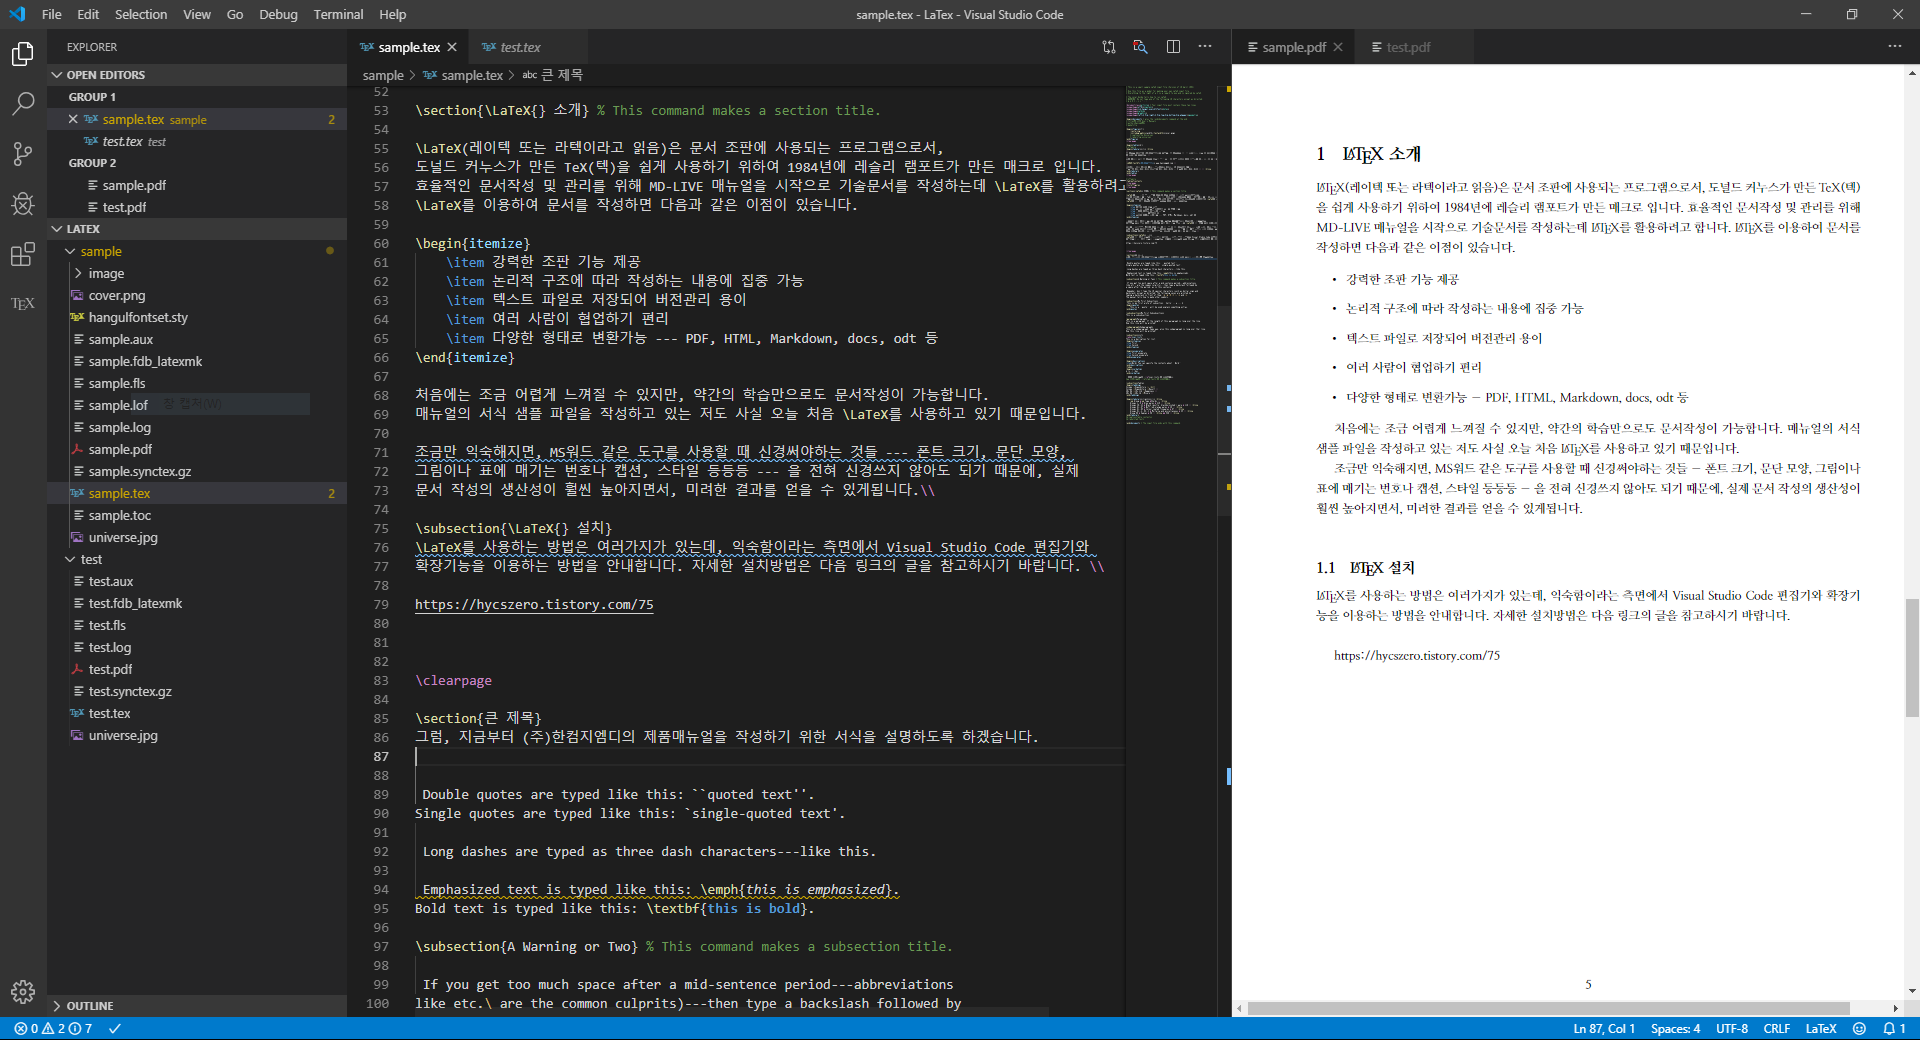
\includegraphics[scale=0.3]{images/chapter1/vscode.png}
    \caption{VS Code를 이용한 \LaTeX 편집}
    \label{fig:vscode}
\end{figure}

\section{\LaTeX{} 참고 자료}
\LaTeX의 기본적인 사용법은 다음 한국TEX사용자그룹(www.ktug.org)의 처음시작하기 문서를 참고하시기 바랍니다. \\

http://wiki.ktug.org/wiki/wiki.php/처음시작하기 \\
\clearpage


    
\chapter{매뉴얼 작성 원칙}
매뉴얼의 본문은 항상 경어체를 사용합니다. 가능한 ``---니다.''로 문장이 끝나도록 작성하고,
``---에요.''와 같은 표현은 사용하지 않도록 주의하시기 바랍니다. 또한, 앞쪽에 작성해 둔 문서의
표기방식을 잘 참조하여, 작성하는 내용에 맞는 표기방식을 사용하시기 바랍니다.\\

본문은 서술형으로 작성하되 다음과 같은 나열 리스트 작성시에는 가급적 개조식으로 작성하시기 바랍니다.
\begin{itemize}
    \item 이 부분은 개조식으로 작성할 것
    \item 각 항목에 대한 설명이 필요할 경우 설명형 리스트를 사용할 것 \\
\end{itemize}

항목별 설명이 필요한 경우 다음과 같은 설명형 리스트를 사용합니다.

\begin{description}
    \item[항목1] 설명도 가급적 개조식으로 작성하는 것을 권장함
    \item[항목2] 부득이한 경우 항목에 대한 설명을 서술식으로 작성합니다.
    \item[항목3] 같은 설명 그룹 안에서는 개조식과 서술식을 혼용하지 말고 통일해서 사용합니다.
\end{description}

    
\chapter{제목 만들기}
새로운 장은 시작하는 가장 큰 제목인 챕터 제목은 다음과 같이 작성합니다.
\begin{verbatim}
\chapter{챕터 제목}
\end{verbatim}
내용 작성

\section{큰 제목}
큰 제목은 다음과 같이 작성합니다.
\begin{verbatim}
\section{큰 제목}
\end{verbatim}
내용 작성

\subsection{중간 제목}
중간 제목은 다음과 같이 작성합니다. 중간 제목까지 자동으로 생성되는 차례에 포함됩니다.
\begin{verbatim}
\subsection{중간 제목}
\end{verbatim}
내용 작성

\subsubsection{작은 제목}
작은 제목은 다음과 같이 작성합니다. 작은 제목 부터는 번호가 붙지 않습니다.
\begin{verbatim}
\subsubsection{작은 제목}
\end{verbatim}
내용 작성

\paragraph{더 작은 제목}
더 작은 제목은 다음과 같이 작성합니다. 더 작은 제목은 설명형 리스트와 유사합니다.
\begin{verbatim}
\paragraph{더 작은 제목}
\end{verbatim}
내용 작성

\subparagraph{가장 작은 제목}
가장 작은 제목은 다음과 같이 작성합니다. 더 작은 제목과 같지만, 약간 들여쓰기가 됩니다.
\begin{verbatim}
\subparagraph{가장 작은 제목}
\end{verbatim}
내용 작성

    
\chapter{문서 만들기} 
본 장에서는 실제 문서를 작성하기 위해 필요한 다양한 명령어들을 소개합니다. 이렇게까지 친절할 필요가
있을까하는 의문이 강하게 듭니다.

\section{본문 내용 작성}
\subsection{글꼴 바꾸기}
\subsubsection{진하게}
\begin{verbatim}
    \textbf{진하게 표시할 글자}
\end{verbatim}

\subsubsection{나눔고딕체 사용}
\begin{verbatim}
    \textsf{나눔고딕체로 표시할 내용}
\end{verbatim}

\subsection{그대로 표시}
표기방식에 설명된 파일/경로명, 사용자 입력 및 소스코드 등은 다음과 같이 작성합니다.
\begin{verbatim}
    \begin{verbatim}
        내용 작성
    \end{vertim}
\end{verbatim}

\subsection{주의 또는 참고사항}
\begin{verbatim}
    \begin{notice}
        내용 작성
    \end{notice}
\end{verbatim}

\section{이미지 넣기}
문서에 그림을 넣는 작업의 간단한 예시입니다. 그림과 관련한 자세한 내용은 아래 링크의 그림넣기 장을
참고하시기 바랍니다. \\

http://willkwon.dothome.co.kr/wp-content/uploads/2018/01/lecture3.pdf

\subsection{이미지 넣기 명령}
\begin{verbatim}
    \begin{figure}[h!]  % t! = top, h! = here, b! = bottom
        \centering            % 이미지 정렬
        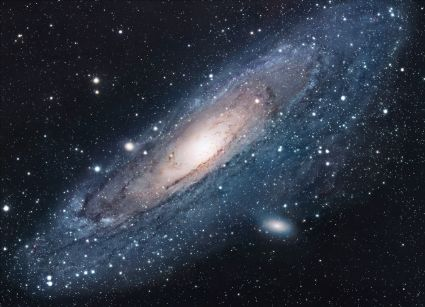
\includegraphics[scale=2]{images/universe}
        \caption{그림 아래에 표시될 캡션}
        \label{fig:universe}   %이미지 참조를 위한 레이블
    \end{figure}
\end{verbatim}

\begin{figure}[h!] 
    \centering            % 이미지 정렬
    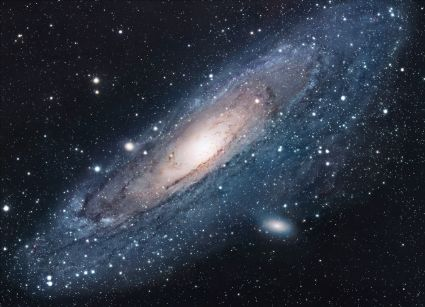
\includegraphics[scale=2]{images/universe}
    \caption{그림 아래에 표시될 캡션}
    \label{fig:universe}   %이미지 참조를 위한 레이블
\end{figure}

\subsection{이미지 레이블 참조}
문서에 넣은 이미지에 대한 레이블은 다음과 같이 참조할 수 있습니다. 이렇게 한 번 작성된 참조는
실제 그림 번호가 바뀌더라도 수정할 필요가 없습니다. 개인적으로 \LaTeX의 최대 장점이라 생각합니다.

\begin{verbatim}
    관련된 내용은 그림 \ref{fig:universe}을 참고하시기 바랍니다. 
\end{verbatim}

관련된 내용은 그림 \ref{fig:universe}을 참고하시기 바랍니다.

\section{표 만들기} 
문서에 표를 작성하는 작업의 간단한 예시입니다. 표 작성과 관련한 자세한 내용은 아래 링크의 표 넣기
장을 참고하시기 바랍니다. \\

http://willkwon.dothome.co.kr/wp-content/uploads/2018/01/lecture3.pdf \\

표를 만드는 작업은 상당히 \LaTeX에서 상당히 까다로운 작업으로 표를 생성해주는 서비스를 이용하는 것도
좋은 방법입니다.

https://www.tablesgenerator.com/

\subsection{표 만들기 명령}
\begin{verbatim}
    \begin{table}
        \begin{tabu}{X | X | X | X} \hline
            \textbf{구분} & \textbf{항목} & \textbf{내용} & \textbf{비고} \\ \hline
                구분1 & 항목1 & 내용1 & 비고1 \\ \hline
                구분2 & 항목2 & 내용2 & 비고2 \\ \hline
            \end{tabu}
            \caption{표에 대한 설명}
            \label{tab:table_01}
    \end{table}
\end{verbatim}

\begin{table}[h!]
    \begin{tabu}{X | X | X | X} \hline
        \textbf{구분} & \textbf{항목} & \textbf{내용} & \textbf{비고} \\ \hline
            구분1 & 항목1 & 내용1 & 비고1 \\ \hline
            구분2 & 항목2 & 내용2 & 비고2 \\ \hline
        \end{tabu}
        \caption{표에 대한 설명}
        \label{tab:table_01}
\end{table}

\subsection{표 레이블 참조}
작성된 표에 대한 레이블도 그림과 동일한 방법으로 참조할 수 있습니다.

\begin{verbatim}
    관련된 내용은 표 \ref{tab:table_01}을 참고하시기 바랍니다. 
\end{verbatim}
관련된 내용은 표 \ref{tab:table_01}을 참고하시기 바랍니다. 

\section{각주 넣기}
문서 내의 특정한 단어 또는 문장에 대한 각주는 다음 명령어를 통해 작성할 수 있습니다.

\begin{verbatim}
    첫 번째 각주와 두 번째 각주입니다.
\end{verbatim}

첫 번째 각주\footnote{각주 안에서 참고나 인용된 문서 등은 기울임 글씨체로 표시합니다.}와
두 번째 각주\footnote{\emph{MD-RED v4.0}을 기대해 주세요.}입니다.

\section{나누어서 작업하기}
하나의 문서를 여러 명이 나누어서 작업하는 경우, 각자 작업할 파일에 작성을 하고, 다음과 같이
마치 C언어의 include처럼 현재 위치에 다른 파일을 불러오기 할 수 있습니다. 

\begin{verbatim}
    
% {}를 붙이면 공백이 한 칸 생김
\chapter{\LaTeX{} 소개} % This command makes a section title.

\LaTeX(레이텍 또는 라텍이라고 읽음)은 문서 조판에 사용되는 프로그램으로서,
도널드 커누스가 만든 TeX(텍)을 쉽게 사용하기 위하여 1984년에 레슬리 램포트가 만든 매크로 입니다.
효율적인 문서작성 및 관리를 위해 MD-LIVE 매뉴얼을 시작으로 기술문서를 작성하는데 \LaTeX를 활용하려고 합니다.
\LaTeX를 이용하여 문서를 작성하면 다음과 같은 이점이 있습니다.

\begin{itemize}
    \item 강력한 조판 기능 제공
    \item 논리적 구조에 따라 작성하는 내용에 집중 가능
    \item 텍스트 파일로 저장되어 버전관리 용이
    \item 여러 사람이 협업하기 편리
    \item 다양한 형태로 변환가능 --- PDF, HTML, Markdown, docs, odt 등
\end{itemize}

\LaTeX는 기존 WYSIWYG 방식의 워드프로세서처럼 문서의 조판형태를 직접지정하며 작성하는 방식이 아니라,
지정된 명령어를 이용하여 문서의 논리적인 구조를 지정해 주는 방식으로 문서를 작성합니다.
처음에는 조금 어렵게 느껴질 수 있지만, 약간의 학습만으로도 문서작성이 가능합니다.
사실, 본 매뉴얼 서식 샘플 파일을 작성하고 있는 저도 오늘 처음 \LaTeX을 사용하고 있기 때문입니다.
조금만 익숙해지면, MS워드 같은 도구를 사용할 때 신경써야하는 것들 --- 폰트 크기, 문단 모양, 
그림이나 표에 매기는 번호나 캡션, 스타일 등등등 --- 을 전혀 신경쓰지 않아도 되기 때문에, 실제 
문서 작성의 생산성이 훨씬 높아지면서, 미려한 결과를 얻을 수 있게됩니다.

\section{\LaTeX{} 설치}
\LaTeX를 사용하는 방법은 여러가지가 있는데, 익숙함이라는 측면에서 Visual Studio Code 편집기와 
확장기능을 이용하는 방법을 안내합니다. 자세한 설치방법은 다음 링크의 글을 참고하시기 바랍니다.

\begin{description}
    \item[Windows 환경] https://hycszero.tistory.com/75
    \item[MacOS 환경] https://prestoxic.blogspot.com/2018/05/visual-studio-code-latex-mac.html
    \item[Linux 환경] 직접 알아서 설치
\end{description}

설명에 따라 설치를 완료하면, 그림 \ref{fig:vscode} 처럼 작성내용과 미리보기를 함께 보면서 문서작성을 할 수 있습니다.
\LaTeX를 활용하는데 있어 지금까지의 가장 큰 어려움은 본문에 삽입하는 그림이 어디에 위치하게 될지를 미리 확인할 수 없고,
조절하기도 힘들다는 점입니다.
이 부분은 추가적인 방법을 찾아봐야 할 것 같습니다.

\begin{figure}[t!]
    \centering
    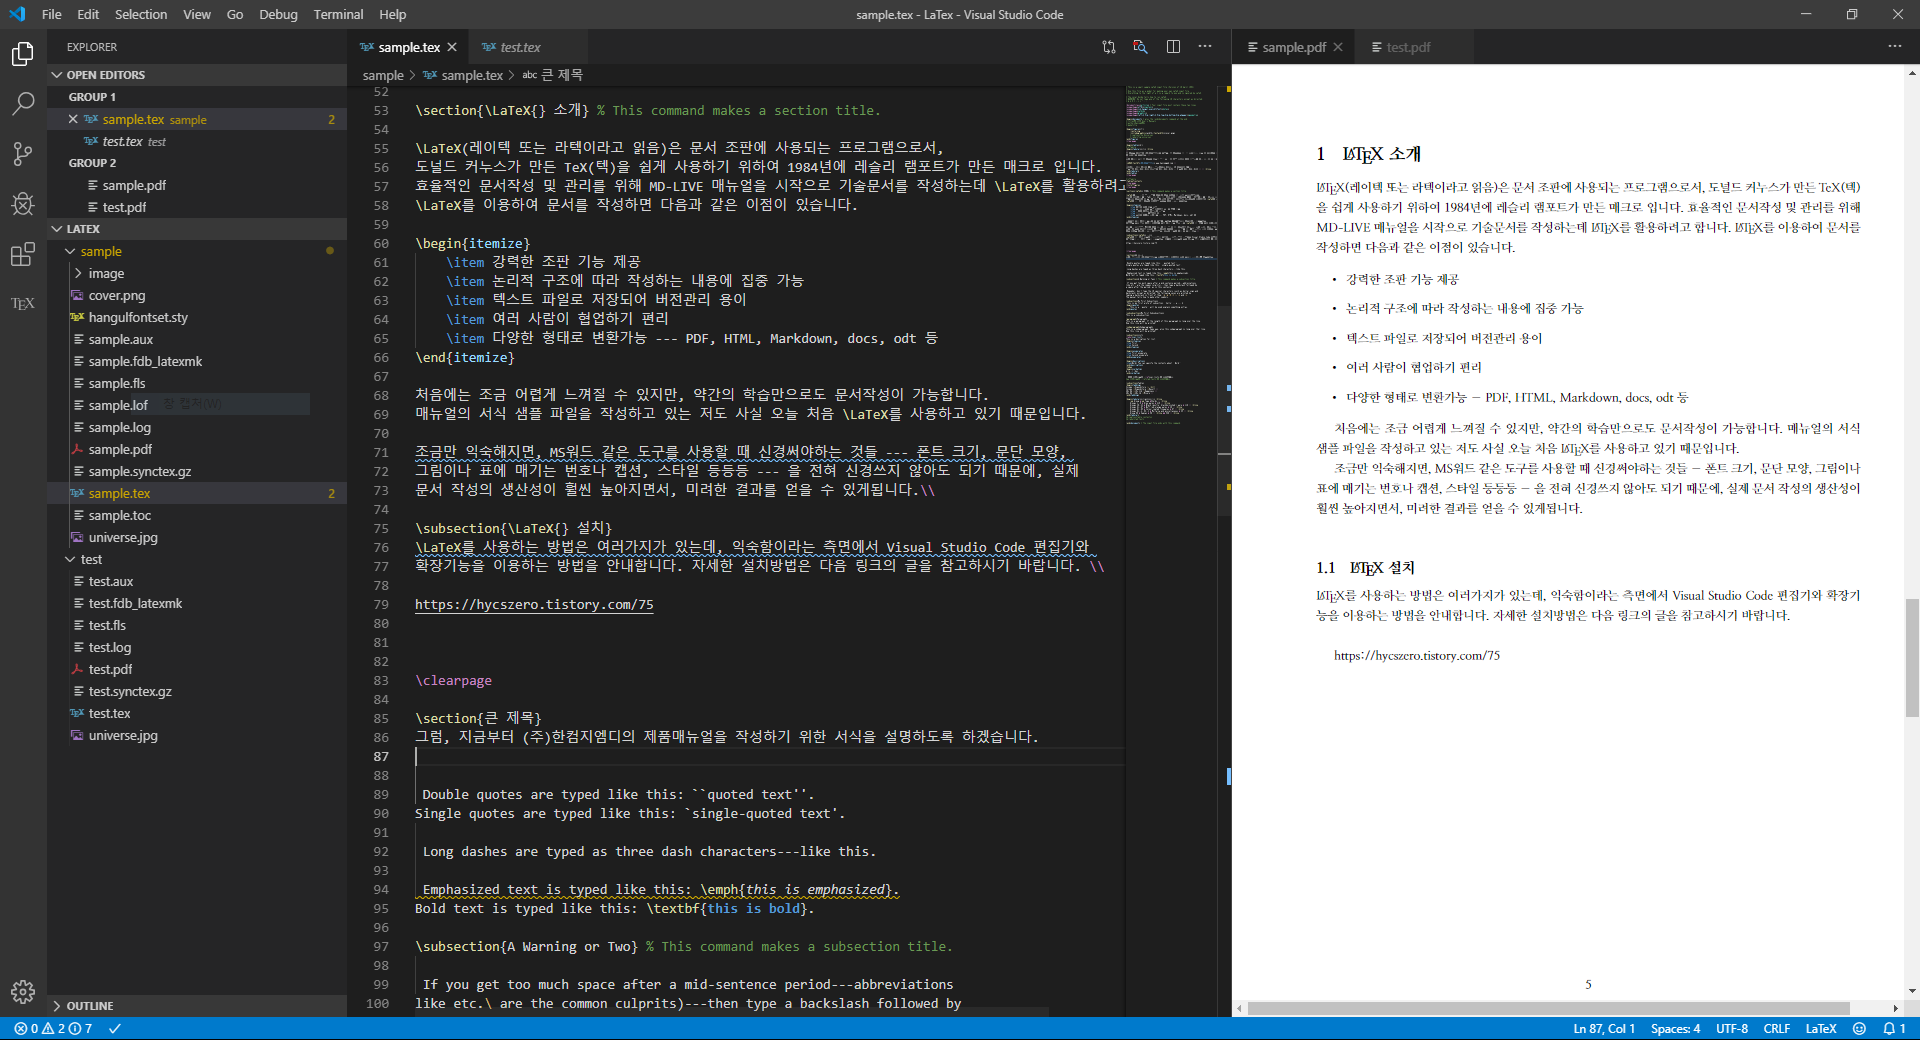
\includegraphics[scale=0.3]{images/chapter1/vscode.png}
    \caption{VS Code를 이용한 \LaTeX 편집}
    \label{fig:vscode}
\end{figure}

\section{\LaTeX{} 참고 자료}
\LaTeX의 기본적인 사용법은 다음 한국TEX사용자그룹(www.ktug.org)의 처음시작하기 문서를 참고하시기 바랍니다. \\

http://wiki.ktug.org/wiki/wiki.php/처음시작하기 \\
\clearpage


    
\chapter{매뉴얼 작성 원칙}
매뉴얼의 본문은 항상 경어체를 사용합니다. 가능한 ``---니다.''로 문장이 끝나도록 작성하고,
``---에요.''와 같은 표현은 사용하지 않도록 주의하시기 바랍니다. 또한, 앞쪽에 작성해 둔 문서의
표기방식을 잘 참조하여, 작성하는 내용에 맞는 표기방식을 사용하시기 바랍니다.\\

본문은 서술형으로 작성하되 다음과 같은 나열 리스트 작성시에는 가급적 개조식으로 작성하시기 바랍니다.
\begin{itemize}
    \item 이 부분은 개조식으로 작성할 것
    \item 각 항목에 대한 설명이 필요할 경우 설명형 리스트를 사용할 것 \\
\end{itemize}

항목별 설명이 필요한 경우 다음과 같은 설명형 리스트를 사용합니다.

\begin{description}
    \item[항목1] 설명도 가급적 개조식으로 작성하는 것을 권장함
    \item[항목2] 부득이한 경우 항목에 대한 설명을 서술식으로 작성합니다.
    \item[항목3] 같은 설명 그룹 안에서는 개조식과 서술식을 혼용하지 말고 통일해서 사용합니다.
\end{description}

    
\chapter{제목 만들기}
새로운 장은 시작하는 가장 큰 제목인 챕터 제목은 다음과 같이 작성합니다.
\begin{verbatim}
\chapter{챕터 제목}
\end{verbatim}
내용 작성

\section{큰 제목}
큰 제목은 다음과 같이 작성합니다.
\begin{verbatim}
\section{큰 제목}
\end{verbatim}
내용 작성

\subsection{중간 제목}
중간 제목은 다음과 같이 작성합니다. 중간 제목까지 자동으로 생성되는 차례에 포함됩니다.
\begin{verbatim}
\subsection{중간 제목}
\end{verbatim}
내용 작성

\subsubsection{작은 제목}
작은 제목은 다음과 같이 작성합니다. 작은 제목 부터는 번호가 붙지 않습니다.
\begin{verbatim}
\subsubsection{작은 제목}
\end{verbatim}
내용 작성

\paragraph{더 작은 제목}
더 작은 제목은 다음과 같이 작성합니다. 더 작은 제목은 설명형 리스트와 유사합니다.
\begin{verbatim}
\paragraph{더 작은 제목}
\end{verbatim}
내용 작성

\subparagraph{가장 작은 제목}
가장 작은 제목은 다음과 같이 작성합니다. 더 작은 제목과 같지만, 약간 들여쓰기가 됩니다.
\begin{verbatim}
\subparagraph{가장 작은 제목}
\end{verbatim}
내용 작성

    
\chapter{문서 만들기} 
본 장에서는 실제 문서를 작성하기 위해 필요한 다양한 명령어들을 소개합니다. 이렇게까지 친절할 필요가
있을까하는 의문이 강하게 듭니다.

\section{본문 내용 작성}
\subsection{글꼴 바꾸기}
\subsubsection{진하게}
\begin{verbatim}
    \textbf{진하게 표시할 글자}
\end{verbatim}

\subsubsection{나눔고딕체 사용}
\begin{verbatim}
    \textsf{나눔고딕체로 표시할 내용}
\end{verbatim}

\subsection{그대로 표시}
표기방식에 설명된 파일/경로명, 사용자 입력 및 소스코드 등은 다음과 같이 작성합니다.
\begin{verbatim}
    \begin{verbatim}
        내용 작성
    \end{vertim}
\end{verbatim}

\subsection{주의 또는 참고사항}
\begin{verbatim}
    \begin{notice}
        내용 작성
    \end{notice}
\end{verbatim}

\section{이미지 넣기}
문서에 그림을 넣는 작업의 간단한 예시입니다. 그림과 관련한 자세한 내용은 아래 링크의 그림넣기 장을
참고하시기 바랍니다. \\

http://willkwon.dothome.co.kr/wp-content/uploads/2018/01/lecture3.pdf

\subsection{이미지 넣기 명령}
\begin{verbatim}
    \begin{figure}[h!]  % t! = top, h! = here, b! = bottom
        \centering            % 이미지 정렬
        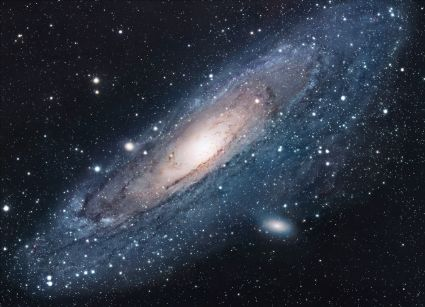
\includegraphics[scale=2]{images/universe}
        \caption{그림 아래에 표시될 캡션}
        \label{fig:universe}   %이미지 참조를 위한 레이블
    \end{figure}
\end{verbatim}

\begin{figure}[h!] 
    \centering            % 이미지 정렬
    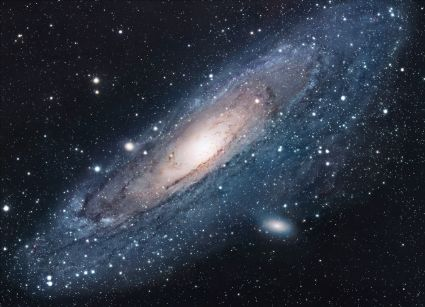
\includegraphics[scale=2]{images/universe}
    \caption{그림 아래에 표시될 캡션}
    \label{fig:universe}   %이미지 참조를 위한 레이블
\end{figure}

\subsection{이미지 레이블 참조}
문서에 넣은 이미지에 대한 레이블은 다음과 같이 참조할 수 있습니다. 이렇게 한 번 작성된 참조는
실제 그림 번호가 바뀌더라도 수정할 필요가 없습니다. 개인적으로 \LaTeX의 최대 장점이라 생각합니다.

\begin{verbatim}
    관련된 내용은 그림 \ref{fig:universe}을 참고하시기 바랍니다. 
\end{verbatim}

관련된 내용은 그림 \ref{fig:universe}을 참고하시기 바랍니다.

\section{표 만들기} 
문서에 표를 작성하는 작업의 간단한 예시입니다. 표 작성과 관련한 자세한 내용은 아래 링크의 표 넣기
장을 참고하시기 바랍니다. \\

http://willkwon.dothome.co.kr/wp-content/uploads/2018/01/lecture3.pdf \\

표를 만드는 작업은 상당히 \LaTeX에서 상당히 까다로운 작업으로 표를 생성해주는 서비스를 이용하는 것도
좋은 방법입니다.

https://www.tablesgenerator.com/

\subsection{표 만들기 명령}
\begin{verbatim}
    \begin{table}
        \begin{tabu}{X | X | X | X} \hline
            \textbf{구분} & \textbf{항목} & \textbf{내용} & \textbf{비고} \\ \hline
                구분1 & 항목1 & 내용1 & 비고1 \\ \hline
                구분2 & 항목2 & 내용2 & 비고2 \\ \hline
            \end{tabu}
            \caption{표에 대한 설명}
            \label{tab:table_01}
    \end{table}
\end{verbatim}

\begin{table}[h!]
    \begin{tabu}{X | X | X | X} \hline
        \textbf{구분} & \textbf{항목} & \textbf{내용} & \textbf{비고} \\ \hline
            구분1 & 항목1 & 내용1 & 비고1 \\ \hline
            구분2 & 항목2 & 내용2 & 비고2 \\ \hline
        \end{tabu}
        \caption{표에 대한 설명}
        \label{tab:table_01}
\end{table}

\subsection{표 레이블 참조}
작성된 표에 대한 레이블도 그림과 동일한 방법으로 참조할 수 있습니다.

\begin{verbatim}
    관련된 내용은 표 \ref{tab:table_01}을 참고하시기 바랍니다. 
\end{verbatim}
관련된 내용은 표 \ref{tab:table_01}을 참고하시기 바랍니다. 

\section{각주 넣기}
문서 내의 특정한 단어 또는 문장에 대한 각주는 다음 명령어를 통해 작성할 수 있습니다.

\begin{verbatim}
    첫 번째 각주와 두 번째 각주입니다.
\end{verbatim}

첫 번째 각주\footnote{각주 안에서 참고나 인용된 문서 등은 기울임 글씨체로 표시합니다.}와
두 번째 각주\footnote{\emph{MD-RED v4.0}을 기대해 주세요.}입니다.

\section{나누어서 작업하기}
하나의 문서를 여러 명이 나누어서 작업하는 경우, 각자 작업할 파일에 작성을 하고, 다음과 같이
마치 C언어의 include처럼 현재 위치에 다른 파일을 불러오기 할 수 있습니다. 

\begin{verbatim}
    
% {}를 붙이면 공백이 한 칸 생김
\chapter{\LaTeX{} 소개} % This command makes a section title.

\LaTeX(레이텍 또는 라텍이라고 읽음)은 문서 조판에 사용되는 프로그램으로서,
도널드 커누스가 만든 TeX(텍)을 쉽게 사용하기 위하여 1984년에 레슬리 램포트가 만든 매크로 입니다.
효율적인 문서작성 및 관리를 위해 MD-LIVE 매뉴얼을 시작으로 기술문서를 작성하는데 \LaTeX를 활용하려고 합니다.
\LaTeX를 이용하여 문서를 작성하면 다음과 같은 이점이 있습니다.

\begin{itemize}
    \item 강력한 조판 기능 제공
    \item 논리적 구조에 따라 작성하는 내용에 집중 가능
    \item 텍스트 파일로 저장되어 버전관리 용이
    \item 여러 사람이 협업하기 편리
    \item 다양한 형태로 변환가능 --- PDF, HTML, Markdown, docs, odt 등
\end{itemize}

\LaTeX는 기존 WYSIWYG 방식의 워드프로세서처럼 문서의 조판형태를 직접지정하며 작성하는 방식이 아니라,
지정된 명령어를 이용하여 문서의 논리적인 구조를 지정해 주는 방식으로 문서를 작성합니다.
처음에는 조금 어렵게 느껴질 수 있지만, 약간의 학습만으로도 문서작성이 가능합니다.
사실, 본 매뉴얼 서식 샘플 파일을 작성하고 있는 저도 오늘 처음 \LaTeX을 사용하고 있기 때문입니다.
조금만 익숙해지면, MS워드 같은 도구를 사용할 때 신경써야하는 것들 --- 폰트 크기, 문단 모양, 
그림이나 표에 매기는 번호나 캡션, 스타일 등등등 --- 을 전혀 신경쓰지 않아도 되기 때문에, 실제 
문서 작성의 생산성이 훨씬 높아지면서, 미려한 결과를 얻을 수 있게됩니다.

\section{\LaTeX{} 설치}
\LaTeX를 사용하는 방법은 여러가지가 있는데, 익숙함이라는 측면에서 Visual Studio Code 편집기와 
확장기능을 이용하는 방법을 안내합니다. 자세한 설치방법은 다음 링크의 글을 참고하시기 바랍니다.

\begin{description}
    \item[Windows 환경] https://hycszero.tistory.com/75
    \item[MacOS 환경] https://prestoxic.blogspot.com/2018/05/visual-studio-code-latex-mac.html
    \item[Linux 환경] 직접 알아서 설치
\end{description}

설명에 따라 설치를 완료하면, 그림 \ref{fig:vscode} 처럼 작성내용과 미리보기를 함께 보면서 문서작성을 할 수 있습니다.
\LaTeX를 활용하는데 있어 지금까지의 가장 큰 어려움은 본문에 삽입하는 그림이 어디에 위치하게 될지를 미리 확인할 수 없고,
조절하기도 힘들다는 점입니다.
이 부분은 추가적인 방법을 찾아봐야 할 것 같습니다.

\begin{figure}[t!]
    \centering
    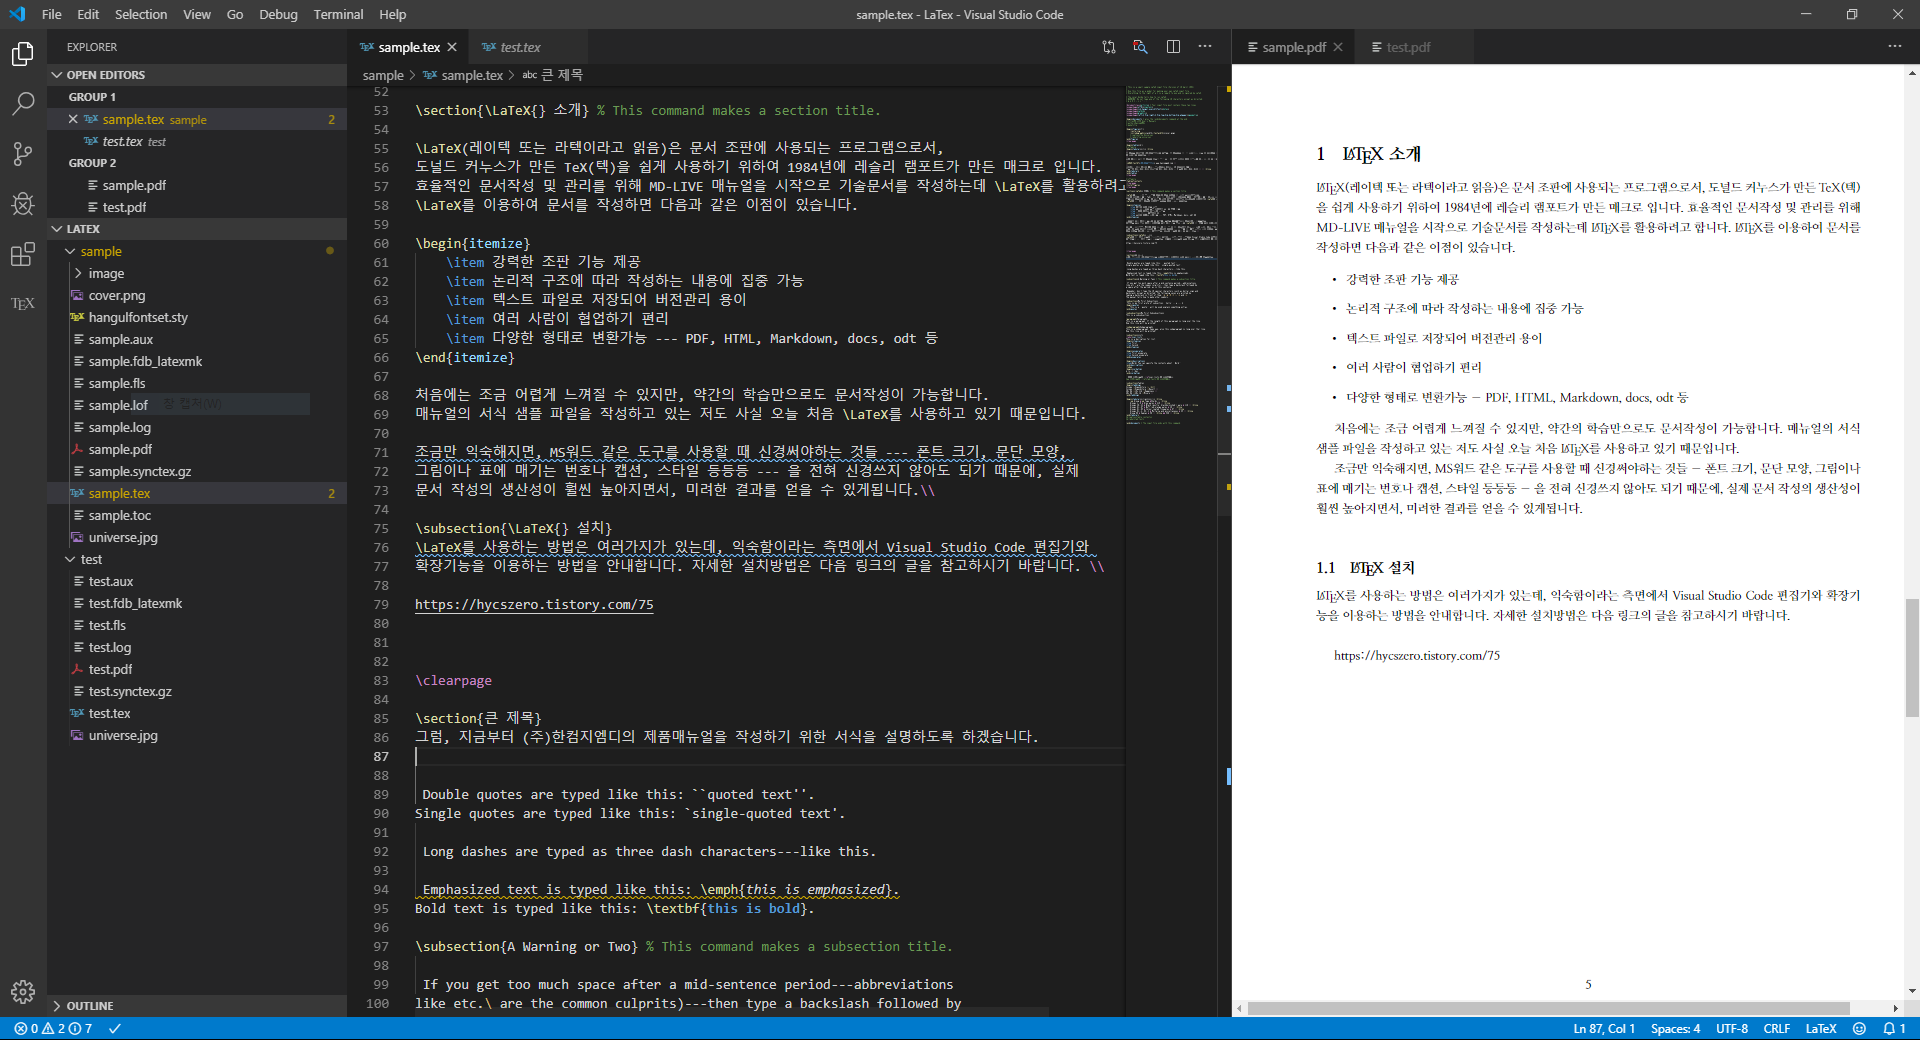
\includegraphics[scale=0.3]{images/chapter1/vscode.png}
    \caption{VS Code를 이용한 \LaTeX 편집}
    \label{fig:vscode}
\end{figure}

\section{\LaTeX{} 참고 자료}
\LaTeX의 기본적인 사용법은 다음 한국TEX사용자그룹(www.ktug.org)의 처음시작하기 문서를 참고하시기 바랍니다. \\

http://wiki.ktug.org/wiki/wiki.php/처음시작하기 \\
\clearpage


    
\chapter{매뉴얼 작성 원칙}
매뉴얼의 본문은 항상 경어체를 사용합니다. 가능한 ``---니다.''로 문장이 끝나도록 작성하고,
``---에요.''와 같은 표현은 사용하지 않도록 주의하시기 바랍니다. 또한, 앞쪽에 작성해 둔 문서의
표기방식을 잘 참조하여, 작성하는 내용에 맞는 표기방식을 사용하시기 바랍니다.\\

본문은 서술형으로 작성하되 다음과 같은 나열 리스트 작성시에는 가급적 개조식으로 작성하시기 바랍니다.
\begin{itemize}
    \item 이 부분은 개조식으로 작성할 것
    \item 각 항목에 대한 설명이 필요할 경우 설명형 리스트를 사용할 것 \\
\end{itemize}

항목별 설명이 필요한 경우 다음과 같은 설명형 리스트를 사용합니다.

\begin{description}
    \item[항목1] 설명도 가급적 개조식으로 작성하는 것을 권장함
    \item[항목2] 부득이한 경우 항목에 대한 설명을 서술식으로 작성합니다.
    \item[항목3] 같은 설명 그룹 안에서는 개조식과 서술식을 혼용하지 말고 통일해서 사용합니다.
\end{description}

    
\chapter{제목 만들기}
새로운 장은 시작하는 가장 큰 제목인 챕터 제목은 다음과 같이 작성합니다.
\begin{verbatim}
\chapter{챕터 제목}
\end{verbatim}
내용 작성

\section{큰 제목}
큰 제목은 다음과 같이 작성합니다.
\begin{verbatim}
\section{큰 제목}
\end{verbatim}
내용 작성

\subsection{중간 제목}
중간 제목은 다음과 같이 작성합니다. 중간 제목까지 자동으로 생성되는 차례에 포함됩니다.
\begin{verbatim}
\subsection{중간 제목}
\end{verbatim}
내용 작성

\subsubsection{작은 제목}
작은 제목은 다음과 같이 작성합니다. 작은 제목 부터는 번호가 붙지 않습니다.
\begin{verbatim}
\subsubsection{작은 제목}
\end{verbatim}
내용 작성

\paragraph{더 작은 제목}
더 작은 제목은 다음과 같이 작성합니다. 더 작은 제목은 설명형 리스트와 유사합니다.
\begin{verbatim}
\paragraph{더 작은 제목}
\end{verbatim}
내용 작성

\subparagraph{가장 작은 제목}
가장 작은 제목은 다음과 같이 작성합니다. 더 작은 제목과 같지만, 약간 들여쓰기가 됩니다.
\begin{verbatim}
\subparagraph{가장 작은 제목}
\end{verbatim}
내용 작성

    
\chapter{문서 만들기} 
본 장에서는 실제 문서를 작성하기 위해 필요한 다양한 명령어들을 소개합니다. 이렇게까지 친절할 필요가
있을까하는 의문이 강하게 듭니다.

\section{본문 내용 작성}
\subsection{글꼴 바꾸기}
\subsubsection{진하게}
\begin{verbatim}
    \textbf{진하게 표시할 글자}
\end{verbatim}

\subsubsection{나눔고딕체 사용}
\begin{verbatim}
    \textsf{나눔고딕체로 표시할 내용}
\end{verbatim}

\subsection{그대로 표시}
표기방식에 설명된 파일/경로명, 사용자 입력 및 소스코드 등은 다음과 같이 작성합니다.
\begin{verbatim}
    \begin{verbatim}
        내용 작성
    \end{vertim}
\end{verbatim}

\subsection{주의 또는 참고사항}
\begin{verbatim}
    \begin{notice}
        내용 작성
    \end{notice}
\end{verbatim}

\section{이미지 넣기}
문서에 그림을 넣는 작업의 간단한 예시입니다. 그림과 관련한 자세한 내용은 아래 링크의 그림넣기 장을
참고하시기 바랍니다. \\

http://willkwon.dothome.co.kr/wp-content/uploads/2018/01/lecture3.pdf

\subsection{이미지 넣기 명령}
\begin{verbatim}
    \begin{figure}[h!]  % t! = top, h! = here, b! = bottom
        \centering            % 이미지 정렬
        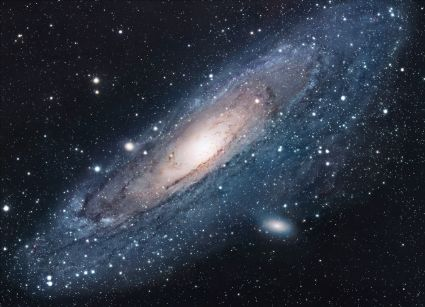
\includegraphics[scale=2]{images/universe}
        \caption{그림 아래에 표시될 캡션}
        \label{fig:universe}   %이미지 참조를 위한 레이블
    \end{figure}
\end{verbatim}

\begin{figure}[h!] 
    \centering            % 이미지 정렬
    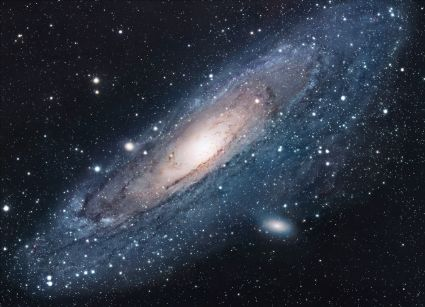
\includegraphics[scale=2]{images/universe}
    \caption{그림 아래에 표시될 캡션}
    \label{fig:universe}   %이미지 참조를 위한 레이블
\end{figure}

\subsection{이미지 레이블 참조}
문서에 넣은 이미지에 대한 레이블은 다음과 같이 참조할 수 있습니다. 이렇게 한 번 작성된 참조는
실제 그림 번호가 바뀌더라도 수정할 필요가 없습니다. 개인적으로 \LaTeX의 최대 장점이라 생각합니다.

\begin{verbatim}
    관련된 내용은 그림 \ref{fig:universe}을 참고하시기 바랍니다. 
\end{verbatim}

관련된 내용은 그림 \ref{fig:universe}을 참고하시기 바랍니다.

\section{표 만들기} 
문서에 표를 작성하는 작업의 간단한 예시입니다. 표 작성과 관련한 자세한 내용은 아래 링크의 표 넣기
장을 참고하시기 바랍니다. \\

http://willkwon.dothome.co.kr/wp-content/uploads/2018/01/lecture3.pdf \\

표를 만드는 작업은 상당히 \LaTeX에서 상당히 까다로운 작업으로 표를 생성해주는 서비스를 이용하는 것도
좋은 방법입니다.

https://www.tablesgenerator.com/

\subsection{표 만들기 명령}
\begin{verbatim}
    \begin{table}
        \begin{tabu}{X | X | X | X} \hline
            \textbf{구분} & \textbf{항목} & \textbf{내용} & \textbf{비고} \\ \hline
                구분1 & 항목1 & 내용1 & 비고1 \\ \hline
                구분2 & 항목2 & 내용2 & 비고2 \\ \hline
            \end{tabu}
            \caption{표에 대한 설명}
            \label{tab:table_01}
    \end{table}
\end{verbatim}

\begin{table}[h!]
    \begin{tabu}{X | X | X | X} \hline
        \textbf{구분} & \textbf{항목} & \textbf{내용} & \textbf{비고} \\ \hline
            구분1 & 항목1 & 내용1 & 비고1 \\ \hline
            구분2 & 항목2 & 내용2 & 비고2 \\ \hline
        \end{tabu}
        \caption{표에 대한 설명}
        \label{tab:table_01}
\end{table}

\subsection{표 레이블 참조}
작성된 표에 대한 레이블도 그림과 동일한 방법으로 참조할 수 있습니다.

\begin{verbatim}
    관련된 내용은 표 \ref{tab:table_01}을 참고하시기 바랍니다. 
\end{verbatim}
관련된 내용은 표 \ref{tab:table_01}을 참고하시기 바랍니다. 

\section{각주 넣기}
문서 내의 특정한 단어 또는 문장에 대한 각주는 다음 명령어를 통해 작성할 수 있습니다.

\begin{verbatim}
    첫 번째 각주와 두 번째 각주입니다.
\end{verbatim}

첫 번째 각주\footnote{각주 안에서 참고나 인용된 문서 등은 기울임 글씨체로 표시합니다.}와
두 번째 각주\footnote{\emph{MD-RED v4.0}을 기대해 주세요.}입니다.

\section{나누어서 작업하기}
하나의 문서를 여러 명이 나누어서 작업하는 경우, 각자 작업할 파일에 작성을 하고, 다음과 같이
마치 C언어의 include처럼 현재 위치에 다른 파일을 불러오기 할 수 있습니다. 

\begin{verbatim}
    \input{sub1.tex}
    \input{sub2.tex}
    \input{sub3.tex}
    \input{sub4.tex}
\end{verbatim}

파일을 분리하여 작업하는 경우, 본인이 작업한 파일만 Commit 할 수 있어 관리가 용이해 집니다.


\end{verbatim}

파일을 분리하여 작업하는 경우, 본인이 작업한 파일만 Commit 할 수 있어 관리가 용이해 집니다.


\end{verbatim}

파일을 분리하여 작업하는 경우, 본인이 작업한 파일만 Commit 할 수 있어 관리가 용이해 집니다.


\end{verbatim}

파일을 분리하여 작업하는 경우, 본인이 작업한 파일만 Commit 할 수 있어 관리가 용이해 집니다.

